\documentclass[12pt]{exam}
\usepackage[phy]{template-for-exam}
\usepackage{tikz,multicol}
\usepackage[margin=0.4in]{geometry}
\usetikzlibrary{shadings,decorations.pathmorphing,arrows.meta,patterns}


\begin{document}
\pagestyle{empty}

\def\mytitle{Ch 3 - 2D Kinematics Test}

\newcommand{\topmatter} {


  \section*{Equations} 

  \hrule

  \vspace{-.5em}

\begin{multicols}{3}
  \begin{center}

    $\vec{v} = \vec{v}_0 + \vec{a} t$
  
    \emph{\footnotesize ``Old Faithful''}
  
  
    $\vec{x} = \vec{x}_0 + \vec{v}_0 t + \frac{1}{2} \vec{a} t^2$
  
    \emph{\footnotesize``The Big Chalupa''}
  

    $\vec{v}^{\,2} = \vec{v}_0^{\,2}+ 2 \vec{a} \cdot 
    \left(\vec{x}-\vec{x}_0 \right)$

    \emph{\footnotesize ``Ain't Got No Time''}

  \end{center}
\end{multicols}

\vspace{-8pt}
\hrule
\vspace{1em}

\begin{minipage}{2.2in}
    \begin{center}
      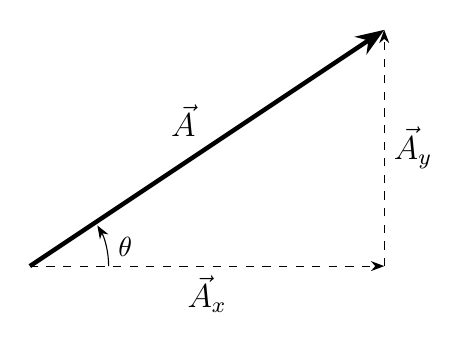
\begin{tikzpicture}[
        every node/.append style={},
        component/.append style={
          dashed,
          -{Stealth}
        },
        resultant/.append style={
          ultra thick,
          -{Stealth}
        },
    ]
      \draw[resultant] 
                (0,0) -- (4.5,3) 
                  node[midway,anchor=south east]{\large $\vec{A}$};
      \draw[component] 
                (0,0) 
                -- (4.5,0) 
                  node[midway,anchor=north]{\large $\vec{A}_x$} ;
      \draw[component] 
                (4.5,0)
                -- (4.5,3) 
                  node[midway,anchor=west]{\large $\vec{A}_y$} ;
      \draw[-Stealth] (1,0) node[anchor=south west]{$\theta$}
                arc[
                  start angle = 0,
                  end angle = 31, 
                  radius = 1
                ];
    \end{tikzpicture}


    \end{center}
  \end{minipage}
  %
  \begin{minipage}{4in}
    \begin{center}
      \begin{align*}
        A_x & = A \cos\theta &
        A_y & = A \sin\theta &
        \theta & = \tan^{-1} \left(\frac{A_y}{A_x}\right)
      \end{align*}

      \hrule 
      
      \begin{align*}
        R &= \frac{v_0^{\,2} \sin\left(2\theta\right)}{g}
      \end{align*}
      \vspace{0em}

      
    \end{center}
  \end{minipage}

  \vspace{1em}

    \hrule

  \begin{align*}
    \vec{v}_{AC} &= \vec{v}_{AB} + \vec{v}_{BC} &
    \vec{v}_{AB} &= -\vec{v}_{BA}
  \end{align*}

  \hrule

}
\newcommand{\bottommatter}{

}

\newcommand{\scantron}[2]{
  \begin{flushright}
  \begin{tikzpicture}
    \node[anchor=south west] at (0,0) {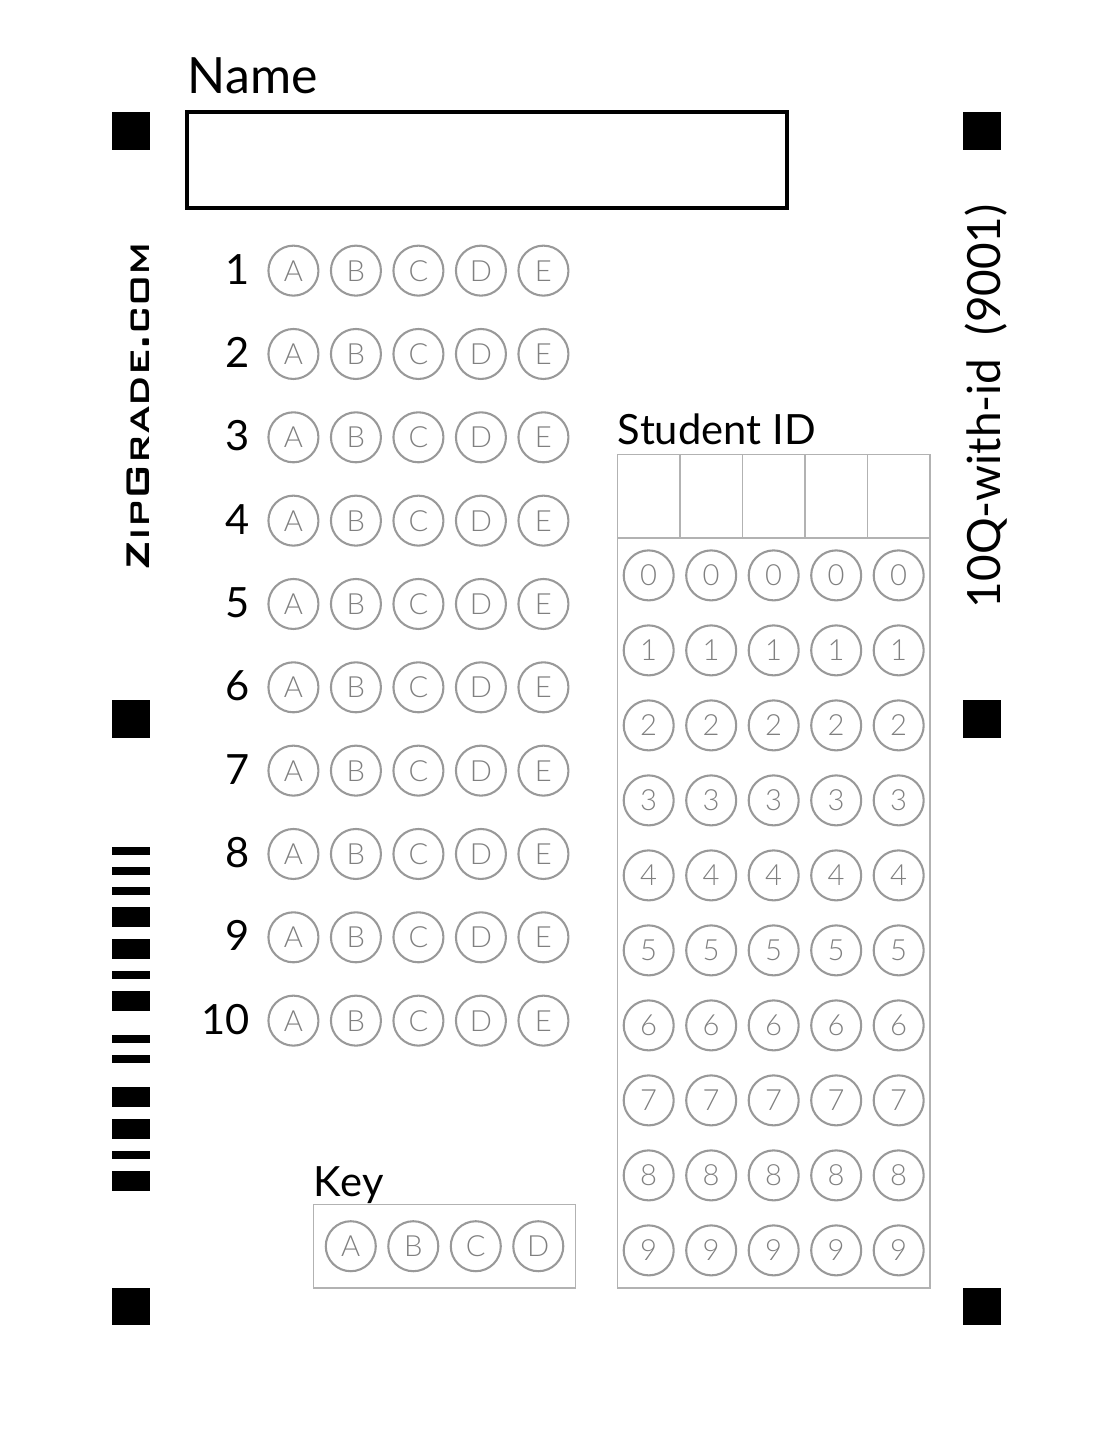
\includegraphics[width=11cm]{10Q.png}};
    \fill (#1,#2) circle (0.28);
    \fill[white] (6,0) rectangle ++(1.45,11);
    \node[fill=white] at (8,10.2) {ZipGrade ID:};
    \node[anchor=west] at (-7.5,13.7) {\Large \bf \sc \mytitle};
  \end{tikzpicture}
\end{flushright}
}



\scantron{3.6}{2.05}
\bottommatter
\topmatter


\pagebreak

\scantron{4.25}{2.05}
\bottommatter
\topmatter

\pagebreak

\scantron{4.85}{2.05}
\bottommatter
\topmatter

\pagebreak
\scantron{5.45}{2.05}
\bottommatter
\topmatter


\end{document}